%
% transfer.tex
%
% (c) 2019 Prof Dr Andreas Müller, Hochschule Rapperswil
%
\subsection{Strahlen und Transfermatrizen
\label{mo:subsection:transfermatrizen}}
Wir möchten den Verlauf eines Lichtstrahls durch ein optisches System
berechnen können.
Im Allgemeinen müssen wir dazu dem Strahl durch das optische System
folgen und an jeder Grenzfläche das Brechungsgesetz anwenden um die
Richtung des Strahls nach dem Durchgang durch die Grenzfläche zu
bestimmen.
Natürlich kann man dazu die Methoden der Vektorgeometrie verwenden,
die in Kapitel~\ref{chapter:orthogonalitaet} entwickelt werden.
Da das Brechungsgesetz nicht linear ist, werden die Gleichungen, die
wir zu lösen haben, sehr kompliziert werden und es ist unwahrscheinlich,
dass wir eine Lösung in geschlossener Form werden finden können.

Um zum Beispiel die Brennweite einer Linse zu berechnen, genügt es jedoch,
Strahlen zu verfolgen, die sehr nahe am Zentrum durch die Linse gehen.
Die auftretenden Brechungswinkel sind dann sehr klein und wir können im
Brechungsgesetz statt des Sinus den Winkel (in Bogenmass) verwenden.
Der Zusammenhang zwischen den Winkeln wird damit linear und es ist 
denkbar, dass sich in dieser Näherung das optische System mit Matrizen
beschreiben lässt.

In der Praxis werden optische Systeme aus Linsen gebaut, die 
sphärische Oberflächen haben.
Solche Linsen sind besonders einfach herzustellen.
Daher können uns daher für die Anwendungen auf rotationssymmetrische
optische Systeme beschränken, wo Linsen auf einer gemeinsamen
optischen Achse montiert sind.
Wir können uns für die beabsichtigte Näherung weiter auf Strahlen
beschränken, die in einer Ebene durch die optische Achse verlaufen.

\subsubsection{Parametrisierung von Strahlen}
\begin{figure}
\centering
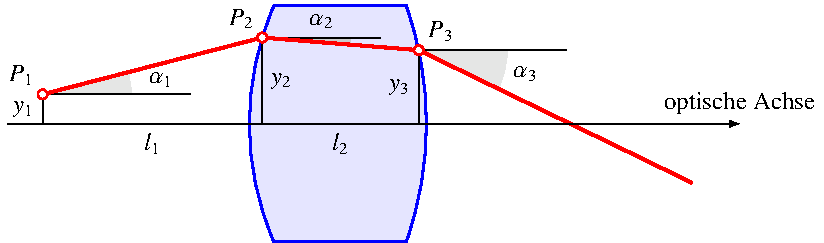
\includegraphics{applications/matrixoptik/ray.pdf}
\caption{Parametrisierung eines Strahls in einem optischen System.
In jedem Punkt wird der Strahl durch den Höhe $y$ über der optischen
Achse und den Winkel $\alpha$ zur optischen Achse beschrieben.
\label{mo:ray}}
\end{figure}
Als erstes müssen wir einen Lichtstrahl im optischen System beschreiben.
In Abbildung~\ref{mo:ray} sind die Punkte hervorgeheben, in denen
die Richtung des Strahls ändert.
Wir können den Strahl rekonstruieren, wenn wir von jedem Punkt den
Abstand $y$ von der optischen Achse kennen sowie den Winkel zur
optischen Achse, unter dem der Strahl den Punkt verlässt.
In der Fachliteratur wird $y$ auch die {\em Höhe} des Strahls über
der optischen Achse genannt.
Den Strahl im Punkt $P_i$ können wir mit dem Vektor
\[
\begin{pmatrix}
y_i\\\alpha_i
\end{pmatrix}
\]
beschreiben.

\subsubsection{Entwicklung entlang der optischen Achse}
Wie hängen die verschiedenen Punkte miteinander zusammen?
Wenn wir dem Strahl, der beim Punkt $P_1$ beginnt, über die Distanz
$l_1$ entlang der optischen Achse folgen, dann ändert sich seine
Höhe über der optischen Achse um $l\sin\alpha_1$.
In der Näherung für kleine Winkel können wir $\sin\alpha_1=\alpha_1$
ersetzen.
Der Winkel des Strahls ändert sich nicht.
Der im Punkt $P_2$ eintreffende Strahl wird also durch den Vektor
\[
\begin{pmatrix}
y_1+l\alpha_1 \\\alpha_1
\end{pmatrix}
\]
beschrieben.
Den Zusammenhang zwischen dem Vektor im Punkt kann durch eine Matrix
beschrieben werden.
Es ist nämlich
\[
\begin{pmatrix}
y_1+l\alpha_1\\\alpha_1
\end{pmatrix}
=
\begin{pmatrix}
1&l\\0&1
\end{pmatrix}
\begin{pmatrix}
y_1\\\alpha_1
\end{pmatrix}
=
T_l
\begin{pmatrix}
y_1\\\alpha_1
\end{pmatrix}
\qquad
\text{mit}
\qquad
T_l
=
\begin{pmatrix}
1&l\\0&1
\end{pmatrix}.
\]

\begin{definition}
Die Matrix
\begin{equation}
T_l
=
\begin{pmatrix}
1&l\\0&1
\end{pmatrix}
\end{equation}
beschreibt also, wie sich ein Strahl über die Distanz
$l$ entwickelt.
\end{definition}

\subsubsection{Brechung}
Im Punkt $P_2$ in Abbildung~\ref{mo:ray} ändert der Strahl seine
Richtung.
Das Brechungsgesetz beschreibt, wie sich der Winkel ändert.
So wie die Matrix $T_l$ den Zusammenhang der den Strahl beschreibenden
Vektoren über die Distanz $l$ wiedergibt, sollte sich auch eine
Matrix finden lassen, welche den Zusammenhang zwischen dem ankommenden
und dem abgehenden Strahl wiedergeben kann.
Diese Matrix wird von den Brechungsindizes $n_1$ und $n_2$ und vom
Krümmungsradius $R$ der brechenden Fläche abhängen, 
\[
\begin{pmatrix}
y_2\\\alpha_2
\end{pmatrix}
=
B(n_1,n_2,R)
T_l
\begin{pmatrix}
y_1 \\ \alpha_1
\end{pmatrix},
\]
$B(n_1,n_2,R)$ ist die gesuchte Matrix.
Da im Brechungsgesetz nur der Quotient $n_2/n_1$ eingeht, sollte das
auch für $B(n_1,n_2,R)$ der Fall sein.

Um eine Formel für $B(n_1,n_2,R)$ herzuleiten, untersuchen wir die
in Abbildung~\ref{mo:Bmatrix} dargestellte Situation.
Ein Lichtstrahl trifft im Punkt $P$ mit einem Winkel $\alpha_1$
auf die brechende Fläche auf und verlässt ihn mit dem Winkel $\alpha_2$.
Die Höhe ist natürlich für den ankommenden und den abgehenden Strahl
gleich: $y=y_1=y_2$.

\begin{figure}
\centering
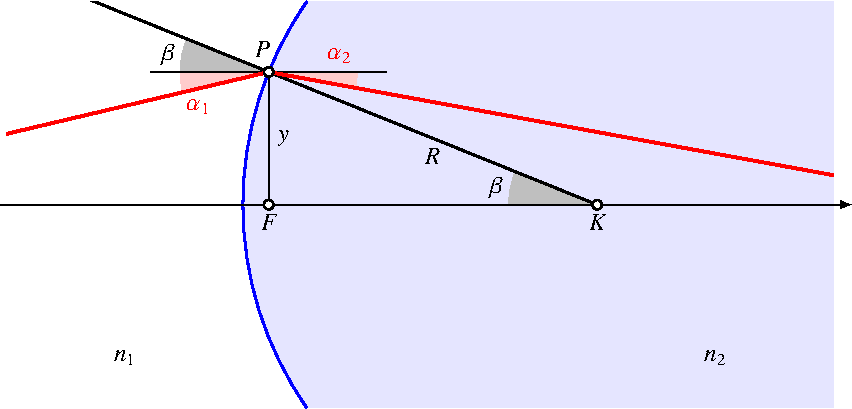
\includegraphics{applications/matrixoptik/curve.pdf}
\caption{Anwendung des Brechungsgesetzes auf die Brechung an einer
sphärischen Fläche.
\label{mo:Bmatrix}}
\end{figure}
Für das Brechungsgesetz sind die Winkel zur Normalen im Punkt $P$
massgebend.
Der Strahl kommt an unter dem Winkel $\beta+\alpha_1$, er verlässt den
Punkt unter dem Winkel $\beta+\alpha_2$ zur Normalen.
Den Winkel $\beta$ können wir im rechtwinkligen Dreieck $\triangle PFK$
ablesen.
Es gilt 
\[
\sin \beta = \frac{y}{R} \simeq \beta.
\]
Das Brechungsgesetz besagt dann
\[
\frac{n_1}{n_2}
=
\frac{\beta+\alpha_2}{\beta+\alpha_1}
\qquad\Rightarrow\qquad
\alpha_2
=
\frac{n_1}{n_2}(\beta+\alpha_1)
-\beta
=
\biggl(
\frac{n_1}{n_2}-1
\biggr)
\frac{y}{R}
+
\frac{n_1}{n_2}\alpha_1
=
\frac{1}{R}
\biggl(
\frac{n_1}{n_2}-1
\biggr)
y
+
\frac{n_1}{n_2}\alpha_1.
\]
Den Zusammenhang zwischen $y_1$, $\alpha_1$, $y_2$ und $\alpha_2$ lässt
sich auch als Matrix schreiben:
\[
\begin{pmatrix}
y_2\\\alpha_2
\end{pmatrix}
=
\begin{pmatrix}
y_1
\\
\displaystyle\frac{1}{R}\biggl(\frac{n_1}{n_2}-1\biggr) y_1
	+ \frac{n_1}{n_2}\alpha_1
\end{pmatrix}
=
\underbrace{
\begin{pmatrix}
1&0\\
\displaystyle\frac{1}{R}\biggl(\frac{n_1}{n_2}-1\biggr)
	& \displaystyle\frac{n_1}{n_2}
\end{pmatrix}
}_{\displaystyle =B(n_1,n_2,R)}
\begin{pmatrix}y_1\\\alpha_1\end{pmatrix}.
\]

\begin{definition}
Die Brechung an einer sphärischen Fläche zwischen Medien mit Brechungsindex
$n_1$ und $n_2$ mit Krümmungsradius $R$ wird beschrieben durch die Matrix
\begin{equation}
B(n_1,n_2,R)
=
B(\nu,R)
=
\begin{pmatrix}
1&0\\
\displaystyle\frac{1}{R}\biggl(\frac{n_1}{n_2}-1\biggr)
	& \displaystyle\frac{n_1}{n_2}
\end{pmatrix}
=
\begin{pmatrix}
1                  & 0  \\
\frac{1}{R}(\nu-1) & \nu
\end{pmatrix}
\label{om:Bn1n2R}
\end{equation}
wobei $\nu = n_1/n_2$ das Verhältnis der Brechungsindizes ist.
\end{definition}

Wie angedeutet hängt $B(n_1,n_2,R)$ nur vom Verhältnis der Brechungsindizes ab.

\subsubsection{Spezialfälle}
Die Matrix $B(\nu,R)$ muss die Brechung an einer Fläche auch in Extremfällen
beschreiben, die wir in diesem Abschnitt untersuchen wollen.

Eine ebene Fläche müsste das Brechungsgesetz reproduzieren.
Eine solche entspricht einem unendlich grossen Krümmungsradius, also
\[
B(\nu,\infty)
=
\begin{pmatrix}
1&0\\0&\nu
\end{pmatrix}.
\]
Diese Matrix besagt, dass
\[
\alpha_2 = \nu \alpha_1 = \frac{n_1}{n_2}\alpha_1
\qquad\Rightarrow\qquad
\frac{\alpha_2}{\alpha_1}=\frac{n_1}{n_2},
\]
dies ist das Brechungsgesetz.

Wenn die Medien auf beiden Seiten der Fläche die gleiche optische
Dichte haben, dann sollte gar keine Brechung stattfinden.
Dies ist der Fall $\nu=1$, in dem die Matrix
\[
B(\nu,R)
=
\begin{pmatrix}
1&0\\
0&1
\end{pmatrix}
\]
die Einheitsmatrix ist, die den Vektor nicht ändert.

\subsubsection{Optische Systeme}
Ein optisches System ist eine Folge von $n$ sphärischen Flächen mit
Krümmungsradius $R_i$, welche Medien mit dem Verhältnis $\nu_i$
der optischen Dichten trennt und an der Position $x_i$ auf der optischen
Achse montiert sind.
Wir verfolten einen Strahl, der im Punkt $(x_0,y_0)$ mit einem Winkel
$\alpha_0$ abgeht.
Dazu muss jeweils eine Matrix der Form $T_l$ mit $l={x_{i+1}-x_{i}}$
angewendet um zu bestimmen, wie sich der Strahl zwischen den Flächen
$i$ und $i+1$ entwickelt.
An der Fläche $i$ muss die Matrix $B(\nu_i,R_i)$ angewendet werden, um
die Brechung des Strahls zu bestimmen.
Die Wirkung des optischen Systems ist daher gegeben durch die Matrix
\[
T
=
T_{x-x_n}
B(\nu_n,R_n)
T_{x_n-x_{n-1}}
\dots
B(\nu_2,R_2)
T_{x_2-x_1}
B(\nu_1,R_1)
T_{x_1-x_0}.
\]
Sie berechnet wie ein an der Koordinaten $x_0$ auf der optischen Achse
abgehender Strahl an der Koordinate $x$ auf der optischen Achse
ankommt.

In den folgenden Abschnitten soll dieses Prinzip für die Berechnung
einfacher optischer Systeme angewendet werden.



